\chapter{Unparse Algorithmus}

\section{Variation-Tree und Variation-Diff}

Um verstehen zu können wie wir Variation-Trees und Variation-Diffs unparsen können, müssen wir uns näher mit dehnen befassen. Damit wir dessen Einschränkungen und Möglichkeiten verstehen.\\


Um Variation-Trees und Variation-Diffs kennenzulernen, betrachten wir zunächst die Definition der Datenstrukturen aus dem Schreiben Classifying Edits to Variability in Source Code~\cite{BTS+:ESECFSE22}.
\begin{definition}
	Ein \textsc{Variation-Tree}  $(V,E,r,\tau,l)$ ist ein Baum mit Knoten $V$, Kanten $E \subseteq V \times V$ und Wurzelknoten $r \in V$. Jede Kante $(x,y) \in E$ verbindet einen Kinderknoten $x$ mit seinem Elternknoten $y$, bezeichnet mit $p(x) = y$. Der Knotentyp $\tau(v) \in $ \{\textsc{artifact,mapping,else}\} identifiziert einen Knoten $v \in V$ entweder als Vertreten einer Implementierungsartefakts, einer Merkmalszuordnung oder einen else-Zweig. Der Label $l(v)$ ist eine aussagenlogische Formel, wenn $\tau(v) =$ \textsc{mapping}, ein Verweis auf ein Implementierungsartefakt, wenn $\tau(v) = $ \textsc{artifact}, oder leer, wenn $\tau(v) =$ \textsc{else} ist. Der Wurzelknoten $r$ hat den Typ $\tau(r) =$ \textsc{mapping} und das Label $l(r) = $ \textsc{true}. Ein Knoten $e$ von Typ $\tau(e) =$ \textsc{else} kann nur unterhalb eines Nichtwurzelknotens $v$ mit dem Typ $\tau(v) =$ \textsc{mapping} platziert, dabei hat ein Knoten $w$ von Typ $\tau(w) =$ \textsc{mapping} höchstens einen Knoten $u$ von dem Typ $\tau(u) =$ \textsc{else}.
\end{definition}
\begin{definition}
	Ein \textsc{Variation-Diff} ist ein gerichteter, zusammenhängender, azyklischer Graph $D=(V,E,r,\tau,l,\Delta) $, welcher einen Wurzelknoten hat, mit Knoten $V$, Kanten $E \subseteq V \times V$, Wurzelknoten $r \in V$, Knotentyp $\tau$, Knotenlabel $l$ und einer Funktion $\Delta : V \cup E \to $\{\textcolor{green}{+},\textcolor{orange}{--},\textcolor{gray}{$\circ$}\}, die definiert, ob ein Knoten oder eine Kante hinzugefügt \textcolor{green}{+} wurde, entfernt \textcolor{orange}{--} wurde oder unverändert \textcolor{gray}{$\circ$} geblieben ist, so das \textsc{project}($D,t$) ein Variation-Tree für alle Zeiten $t \in \{\textcolor{green}{a},\textcolor{orange}{b}\}$ ist.
\end{definition}
\begin{definition}
	Die Projektion \textsc{project}($D,t$) für das Variation-Diff aus Definition 3.2 ist das Entfernen von $\Delta$ und den Knoten und Kanten, welche zu der Zeit t nicht vorhanden sind. \textsc{project}$((V,E,r,\tau,l,\Delta),t) := (\{v \in V | $\textsc{exists}$(t,\Delta(v))\},\{e \in E | $\textsc{exists}$(t,\Delta(e))\},r,\tau,l)$
\end{definition}
Ob ein Knoten oder eine Kante zu einer gegebenen Zeit existiert oder nicht, definieren wir für alle Definitionen, die das Verwenden gleich. Unsere Definition von \textsc{exists} entspricht der Definitionen aus dem Schreiben Classifying Edits to Variability in Source Code~\cite{BTS+:ESECFSE22} und der Bachelorarbeit Constructing Variation Diffs Using Tree Diffing Algorithms~\cite{Moosherr23}
\begin{definition}
	Ob ein Knoten oder eine Kante zu einer gegebenen Zeit existiert oder nicht, stellt \textsc{exists}  für $x \in V \cup E$ das folgendermaßen fest \textsc{exists}$(t,\Delta(x)) := (t = \textcolor{orange}{b} \land \Delta(x) \neq \textcolor{green}{+}) \lor (t = \textcolor{green}{a} \land \Delta(x) \neq \textcolor{orange}{-})$
\end{definition}

In der Abbildung unten ist ein Beispiel für ein Variation-Diff gegeben, damit man sich besser darunter vorstellen kann. Es hilf auch bei dem Verständnis von Variation-Trees da diese, ähnlich zu dem Variation-Diffs sind. Die Abbildung zeigt wie die unterschiedlichen Komponenten des Variation-Diffs visuell dargestellt werden können. Diese Darstellung wurde an der Darstellung eines Variation-Diffs aus DiffDetective angelehnt, aber entspricht der nicht ganz.
\begin{tikzpicture}
	\node[draw,diamond,fill=lightgray,thick] {root}
	child {node[draw,circle,thick,fill=green] {foo()}}
	child {node[draw,rectangle,thick,fill=green] {\textbf{if} B}
		child {node[draw,rectangle,thick] {\textbf{if} A$\lor$C}
			child { node[draw,circle,thick] {bar()}}
			child { node[draw,ellipse,thick] {\textbf{else}}
				child { node[draw,circle,thick,fill=green] {baz()}}
				child { node[draw,circle,thick,fill=red] {ban()}}
			}
		}
		child { node[draw,circle,thick] {boo()}}
	};
	\node[draw] (a) at (4,0) {einige Knoten aus $V$};
	\draw[->] (a) -- (1,0);
	\draw[->] (a) -- (1.2,-1.1);
	\draw[->] (a) -- (1.9,-2.2);
	\node[draw] (b) at (6,-1.5) {einige Kanten aus $E$};
	\draw[->] (b) -- (0.8,-0.8);
	\draw[->] (b) -- (1.1,-2);
	\node[draw] (c) at (-4,0)  {Wurzelknoten $r$};
	\draw[->] (c) -- (-1,0);
	\node[draw,align=center] (d) at (-4,-1.2)  {$\Delta$ ist $+$ \\ Knoten ist grün};
	\draw[->] (d) -- (-1.5,-1.3);
	\node[draw,align=center] (e) at (-4,-2.7)  {$\tau$ ist \textsc{mapping} \\ Knoten ist rechteckig};
	\draw[->] (e) -- (-1,-3);
	\node[draw] (f) at (-4,-3.7)  {Label ist A$\lor$C};
	\draw[->] (f) -- (-1,-3.1);
	\node[draw] (g) at (-4,-4.5)  {Label ist bar()};
	\draw[->] (g) -- (-1.5,-4.5);
	\node[draw,align=center] (h) at (-4,-5.5)  {$\tau$ ist \textsc{artifact} \\ Knoten ist rund};
	\draw[->] (h) -- (-1,-6);
	\node[draw,align=center] (i) at (6,-3)  {$\Delta$ ist $\circ$ \\ Knoten ist weis};
	\draw[->] (i) -- (2.3,-3);
	\node[draw,align=center] (j) at (6,-4.5)  {$\tau$ ist \textsc{else} \\ Knoten ist elliptisch};
	\draw[->] (j) -- (1.5,-4.5);
	\node[draw,align=center] (k) at (6,-6)  {$\Delta$ ist $-$ \\ Knoten ist rot};
	\draw[->] (k) -- (2.3,-6);
\end{tikzpicture}


Das ist aber nicht die einzige Möglichkeit Variation-Tree und Variation-Diff zu definieren. In der Bachelorarbeit  Constructing Variation Diffs Using Tree Diffing Algorithms~\cite{Moosherr23} wurden die Variatio-Tree und Variation-Diff etwas anders definiert. Obwohl dort auch Variation-Tree und Variation-Diff definiert werden, werden wir in dieser Arbeit die Definitionen aus Constructing Variation Diffs Using Tree Diffing Algorithms als geordneter Varaition-Tree und als geordneter Varaition-Diff bezeichnen. Diese Definitionen haben eine Eigenschaft, welche wir brauchen um das Unparsen zu bewerkstelligen. Das ist die Ordnung der Kinderknoten ohne, die wir nicht eindeutig wissen, wie der Inhalt der Knoten einzuordnen ist. Genauerer gehen wir darauf in Unterkapitel 3.3 Verlorengehende Informationen. Die Definitionen von geordneten Variation-Trees und geordneten Variation-Diff sehen wie folgt aus:
\begin{definition}
	Ein \textsc{geordneter Variation-Tree} (V,E,r,$\tau$,l,O) ist ein geordneter Baum mit einem Wurzelknoten r $\in$ V, mit Knoten V, Kanten E $\subseteq$ V $\times$ V, Knotentypen $\tau$ : V $\rightarrow$ \{\textsc{artifact,mapping,else}\}, Label l : V $\rightarrow$ A $\cup$ P, wobei A die Menge aller Artefakte ist und P die Menge aller aussagenlogischer Formeln und eine injektive Funktion O : V $\rightarrow$  $\mathbb{N}$, die eine Ordnung für die Kinder eines jeden Knotens jedes Knotens definiert. Der Wurzelknoten r muss den Typ $\tau$(r) = \textsc{mapping} und Label l(r) = true haben. Ein Knoten v mit $\tau$(v) = \textsc{artifact} wird als Artefaktknoten und muss ein Artefakt a $\in$ A als Label l(v) = a haben. Analog dazu wird ein Knoten v mit $\tau$(v) = \textsc{mapping} als Mappingknoten bezeichnet und muss eine Merkmals-Abbildung, eine propositionale Formel p $\in$ P als Label l(v) = p haben. Im Gegensatz dazu hat ein Knoten v mit $\tau$(v) = \textsc{else} ein leeres Label, wird als else-Knoten bezeichnet und muss der einzige else-Knoten eines if-Knotens sein. 
	
\end{definition}
	

\begin{definition}
	Ein \textsc{geordneter Variation-Diff} $D=(V,E,r,\tau,l,\Delta,O_{before},O_{after}) $ ist ein gerichteter, zusammenhängender, azyklischer Graph, welcher einen Wurzelknoten hat, mit Koten V, Kanten $E \subseteq V \times V$, Wurzelknoten r $\in$ V, Knotentypen $\tau$ : V $\rightarrow$ \{\textsc{artifact,mapping,else}\}, Label l : V $\rightarrow$ A $\cup$ P, wobei A die Menge aller Artefakte ist und P die Menge aller aussagenlogischer Formeln, die Zeit der Existenz $\Delta : V \cup E \rightarrow $\{+,--,$\circ$\}, die definiert, ob ein Knote oder eine Kante hinzugefügt + wurde, entfernt -- wurde oder unverändert $\circ$ geblieben ist, die Kinderknoten vor der Änderung $O_{before}$ und nach der Änderung $O_{after}$ sind eine injektive Funktion $O_{before},O_{after}$ : V $\rightarrow$ $\mathbb{N}$. Die Projektionen  \textsc{$project_{O}$}($D,t$) müssen für alle Zeiten  $t \in \{after,before\}$ ein Variation-Tree mit demselben Wurzelknoten sein.
	
\end{definition}

Für eindeutigkeitshalber haben wir auch die Projektion umbenannt, da sich die Definition von \textsc{$project_{O}$}($D,t$) von der Definition der Projektion \textsc{project}($D,t$) aus der Difinition 3.3 unterscheidet, wegen den zusätzlichen Information, die gespeichert werden. 

\begin{definition}
	Die Projektion \textsc{$project_O$}($D,t$) eines geordneten Variation-Diff \\$D=(V,E,r,\tau,l,\Delta,O_{before},O_{after}) $ zum Zeitpunkt $t \in \{after,before\}$ ist definiert als:\\ \textsc{$project_O$}($D,t$) := $(V',E',r,\tau|_V,l|_V,O_t)$, wobei V' = \{v $\in$ V | \textsc{exists}$(t,\Delta(v))\}$, E' = $\{e \in E | $\textsc{exists}$(t,\Delta(e))\}$ und die Existenz von d $\in$ \{+,--,$\circ$\}, zu der Zeit $t \in \{after,before\}$ ist in der Definition 3.4 gegeben.
\end{definition}

Die Definitionen von normalen Variation-Tree und Variation-Diff sind sehr ähnlich zu den Definitionen von geordneten Variation-Tree und Variation-Diff. Wir sehen hier die Möglichkeit geordnete Variation-Tree bzw. Variation-Diff in normale Variation-Tree bzw. Variation-Diff umzuwandeln. Dazu verwenden wir die Funktionen $reduce_{OVT}$ und $reduce_{OVD}$, dabei wandelt $reduce_{OVT}$ geordneter Variation-Tree zu Variation-Tree, welches wie folgt aussieht $reduce_{OVT}((V,E,r,\tau,l,O)) := (V,E,r,\tau,l)$ und $reduce_{OVD}$ wandelt geordneter Variation-Diff zu Variation-Diff um , wie folgt $reduce_{OVD}((V,E,r,\tau,l,\Delta,O_{before},O_{after})) := (V,E,r,\tau,l,\Delta)$. Es bleibt uns nur noch zu zeigen, dass die Reihenfolge der Anwendung nicht von Bedeutung ist.
\begin{lemma}
	Für ein geordneten Variation-Diff D und eine Zeit $t \in \{before, after\}$ gilt $reduce_{OVT}(project_O(D,t)) = project(reduce_{OVD}(D),t)$.
\end{lemma}
\begin{proof}
	$
	reduce_{OVT}(project_O(D,t))\\ 
	= reduce_{OVT}(project_O((V,E,r,\tau,l,\Delta,O_{before},O_{after}),t))\\
	= reduce_{OVT}((\{v \in V | \textsc{exists}(t,\Delta(v))\},\{e \in E | \textsc{exists}(t,\Delta(e))\},r,\tau,l,O_t))\\
	= (\{v \in V | \textsc{exists}(t,\Delta(v))\},\{e \in E | \textsc{exists}(t,\Delta(e))\},r,\tau,l)\\ 
	= project((V,E,r,\tau,l,\Delta),t)\\ 
	= project(reduce_{OVD}(V,E,r,\tau,l,\Delta,O_{before},O_{after}),t)\\ 
	= project(reduce_{OVD}(D),t)\\
	$
\end{proof}




Jetzt haben wir uns mit dem Beschäftigt wie Variation-Tree und Variation-Diff zu verstehen sind. Dabei haben wir zwei Definitionen von Variation-Tree bzw. Variation-Diff kennengelernt, die sich sehr ähnlich sind aber auch einen Unterschied haben. Was zu Folge hat das sich gewisse Eigenschaften von den unterscheiden. Dazu haben wir gezeigt das es möglich geordnete Variation-Tree bzw. Variation-Diff in Variation-Tree bzw. Variation-Diff überführen und projizieren in beliebiger Reihenfolge anzuwenden, was die Abbildung 3.1 ergibt. Im späteren Verlauf können wir bei Bedarf diese Unterschiede für unsere Zwecke verwenden. Um zu verstehe welche Definition für uns die Angemessenere ist, also welche sich besser für das Unparsen eignet.

\begin{figure}[H]
	\centering
	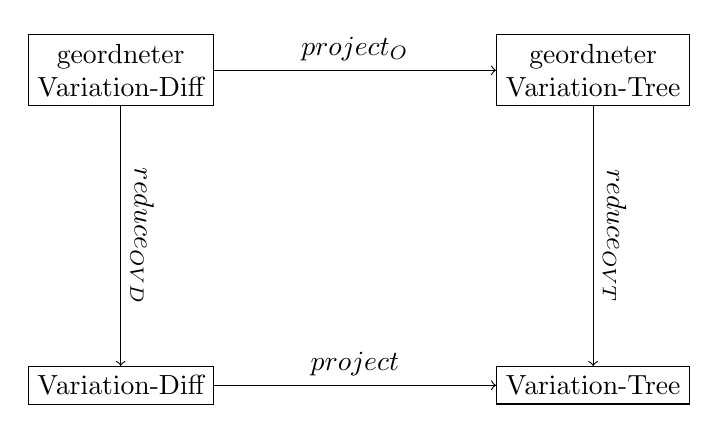
\begin{tikzpicture}
	\node[draw,align=center] (A) at (0,0) {geordneter\\
	Variation-Diff};
	\node[draw,align=center] (B) at (6,0) {geordneter\\
		Variation-Tree};
	\node[draw,align=center] (C) at (0,-4) {Variation-Diff};
	\node[draw,align=center] (D) at (6,-4) {Variation-Tree};
	\draw[->] (A) -- (B)  node[midway,sloped,above] {$project_O$} ;
	\draw[->] (C) -- (D)  node[midway,sloped,above] {$project$} ;
	\draw[->] (A) -- (C)  node[midway,sloped,above] {$reduce_{OVD}$} ;
	\draw[->] (B) -- (D)  node[midway,sloped,above] {$reduce_{OVT}$} ;
	\end{tikzpicture}
	\caption{Transformationen von geordneten Variation-Diff , geordneten Variation-Tree, Variation-Diff und Variation-Tree}
\end{figure}


\section{Parser}

Jetzt beschäftigen wir uns mit den Parsen, also wie Variation-Trees bzw. Variation-Diffs  aus mit C-Präprozessor-Direktiven annotiertem Code bzw. einem textbasierten Diff von solchem Code erstellt werden. Das Verständnis des Parsens ist, für das Verständnis des Unparsens von Bedeutung, da das Unparsen das Parsen invertiert. Dazu schauen wir uns den Parser-Algorithmus von Viegener~\cite{Viegener21} an, welcher das Parsen von Variation-Diffs aus textbasierten Diffs eingeführt hat.\\


Der unten stehender Algorithmus überführt einen textbasierten Diff in einen Variation-Diff. Dabei werden in dem Algorithmus einige Sachen verwendet, die nicht so in der Definition vorkamen. Einer dieser Sachen ist der Code-Typ dieser stellt dar, welche Rolle die Zeile in dem Diff hat. Es kann die Werte if, elif, else, code, oder endif haben. Bei dem Wert if ist gegeben, dass die Zeile eine der Präprozessor Anweisungen \#if, \#ifdef, oder \#ifndef hat. Bei dem Wert else ist in der Zeile die Präprozessor Anweisungen \#else, bei Wert elif ist  die Präprozessor Anweisungen \#elif und bei Wert endif ist  die Präprozessor Anweisungen \#endif gegeben. Wenn der Wert von Code-Typ code ist, dann enthält die Zeile keine Präprozessor Anweisungen sondern normalen Code. Da Wert elif als Erweiterung betrachtet werden kann, wird auf sie nicht Weiter in unserer Arbeit eingegangen. Der Code-Typ einer Zeile findet auch eine Darstellung in dem Variation-Diff und das ist $\tau$. Der Code-Typ if ist gleich dem Wert if von $\tau$ eines Knotens, der 




%Vieleicht sachen die sich von der Definition Unterscheiden erwähnen z.B Code-Type
 um. Ein Variation-Diff ist ein gerichteter azyklischer Graph. Dieser Graph stellt dabei zeilenbasiert den textbasierten Diff dar. Die Knoten des Graphen werden durch einen Diff-Typ und einen Code-Typ eingeordnet. Diese Informationen werden der Zeile entnommen, die der Knoten repräsentiert. Der Diff-Type kann die Werte add, remove oder none einnehmen. Add bedeutet das diese Zeile hinzugefügt wurde, remove das diese Zeile entfernt wurde und none das die Zeile unverändert geblieben ist. Der Code-Typ kann die Werte if, elif, else, code, oder endif haben. Dabei gibt der Code-Type an, das bei dem Wert if die Zeile eine Anweisung des if-Blocks, dass können die sein, enthält und der Knoten darstellt. Bei dem Wert elif es ist die Anweisung , bei else die Anweisung . Bei dem Wert code des Code-Typs enthält die Zeile Code und der Knoten stellt dies dar. Der Wert endif gibt an das die Zeile die Anweisung enthält, in dem Variation-Diff ist dieser Code-Typ nicht enthalten. Die Knoten des Variation-Diffs haben höchstens zwei Elternknoten. Es gibt einen befor Elternknoten, das ist der Elternknoten, welchen der Knoten vor der Änderung hatte. Dieser Elternknoten gibt den umgebenden Präprozessor-Block vor der Änderung an. Es gibt noch einen after Elternknoten das ist der Elternknoten, welchen der Knoten nach der Änderung hat. Dieser Elternknoten gibt den umgebenden Präprozessor-Block nach der Änderung an. Nur Knoten mit Diff-Typ none haben zwei Elternknoten. Die Knoten mit dem Diff-Typ remove haben nur den befor Elternknoten und die Knoten mit dem Diff-Typ add haben nur after Elternknoten. Dabei kann ein befor Elternknoten nicht den Diff-Typ add haben und ein after Elternknoten nicht den Diff-Typ remove. Der Variation-Diff hat noch einen Knoten welcher keine Widerspiegelung in dem textbasierten Diff enthält, das ist der Wurzelknoten. Der Wurzelknoten repräsentiert den ganzen textbasierten Diff. Er hat als einziger Knoten in dem Variation-Diff kein Elternknoten. Der Wurzelknoten hat immer den Diff-Typ none und den Code-Typ if, dabei ist das Feature-Mapping wahr.



\begin{algorithm}[H]
	\SetAlgoLined
	\DontPrintSemicolon
	\KwData{ein textbasierter Diff}
	\KwResult{ein Variation-Diff}
	initialisiere ein Stack/Keller $before$ mit dem Wurzelknoten\;
	initialisiere ein Stack/Keller $after$ mit dem Wurzelknoten\;
	\;
	\ForEach{Zeile in dem Patch/Diff}{
		$\delta$ $\leftarrow$ identifiziere Diff-Typ der Zeile\;
		$\gamma$ $\leftarrow$ identifiziere Code-Typ der Zeile\;
		$\sigma$ $\leftarrow$ identifiziere relevante Stacks mithilfe von  $\delta$\;
		\;
		\eIf{$\gamma$ = endif}{
		Entferne, solange Knoten von allen Stacks in $\sigma$, bis $\gamma$ = if entfernt wurde\;
		}{
			erstelle einen neuen Knoten mit $\delta$, $\gamma$ und gerichtete Kanten von Elternknoten aus $\sigma$ zu dem neu erstellten Knoten\;
			\If{$\gamma$ $\neq$ code}{
				füge den neuen Knoten $\sigma$ hinzu\;
			}
		}
	}
	\caption{Erstellung eines Variation-Diffs aus einem Patch}
\end{algorithm}
Der Algorithmus arbeitet wie folgt. Ganz am Anfang werden zwei Stacks erstellt und jeweils mit dem Wurzelknoten initialisiert, was in Zeilen 1 und 2 des Algorithmus 1 zu sehen ist. Die Stacks speichern dabei die Elternknoten. Ein Stack speichern die Elternknoten in davor Zustand und der anderer im danach Zustand. Beide Stacks werden mit Wurzelknoten befühlt, welcher den ganzen Diff repräsentiert und hat deshalb als einziger Knoten in Variation-Diff keinen Elternknoten. In Zeile 4 ist eine Schleife zu sehen, welche über alle Zeilen des textbasierten Diffs geht. Dabei wird für jede Zeile zuerst der Diff-Typ $\delta$ in Zeile 5 und dann der Code-Typ $\gamma$ in Zeile 6 ermittelt. In Zeile 7 werden die relevanten Stacks $\sigma$ anhand von Diff-Typ $\delta$ bestimmt, und zwar wie folgt:
\[ \sigma =
\begin{cases}
	\text{Stack } after      &, \quad \delta = \text{add}\\
	\text{Stack } before  &, \quad \delta = \text{remove}\\
	\text{Stacks } befor \text{ und } after &, \quad \delta = \text{none}
\end{cases}
\]
Diese Informationen werden zum einen dazu gebraucht für Algorithmus interne Berechnungen und zum anderen zur Erstellung von Knoten gebraucht. Danach in Zeile 9 kommen wir zu einer if-Abfrage. Wenn der Code-Typ der bearbeiteten Zeile endif entspricht, dann wird aus den relevanten Stacks in $\sigma$ solange Knoten entfernt bis man ein Knoten mit dem Code-Type $\gamma$ if entfernt hat. Falls beide Stacks relevant sind, muss der if-Knoten in beiden Stacks gefunden werden. Dieses Vorgehen ist Notwendig, da wenn eine endif-Anweisung kommt, muss der dazugehörige if-Block oder if-else-Block zu Ende sein. Das führt mit sich das die dazugehörigen if-Knoten und else-Knoten keine Elternknoten mehr sein können und aus den Stacks entfernt werden müssen. Wenn der Code-Typ nicht endif entspricht, kommen wir in den else-Teil ab Zeile 11 des Algorithmus 1. Dort wird zuerst ein neuer Knoten erstellt, dazu unter anderem wird Diff-Typ $\delta$ und Code-Typ $\gamma$ verwendet. Es werden auch Kanten von Elternknoten aus den Stacks von $\sigma$ zu diesen neuen Knoten erstellt. Als Nächstes wird in Zeile 13 überprüft, ob der erstellter Knoten nicht von Code-Typ code ist. Diese Abfrage ist nötig da nur solche Knoten ein Elternknoten sein können. Den Code-Typ endif kann dieser Knoten nicht haben, wegen der if-Abfrage in Zeile 9, welche nicht zulässt, dass ein Knoten mit diesem Typ zu dieser Stelle gelangen kann.  Wenn der Knoten nicht von Code-Typ code ist, dann wird dieser Knoten den relevanten Stacks aus $\sigma$ hinzugefügt, sonst wenn der Knoten, den Code-Type code hat, wird nichts gemacht.\\


Der vorgestellter Algorithmus ist für das Parsen von textbasierten Diffs, welche aus mit C-Präprozessor-Annotierten Code entstanden sind, zu Variation-Diffs ausgelegt aber es ist auch möglich den Algorithmus zum Parsen von C-Präprozessor-Annotiertem Code zu einem Variation-Tree zu verwenden. Wir reduzieren das Problem ein Variation-Tree zu parsen auf das Problem ein Variation-Diff zu parsen. Um das anstellen zu können, müssen wir zwei Sachen beachten. Zuerst wäre da die Anpassung der Eingabe, da wir C-Präprozessor-Annotierten Code haben aber der Algorithmus einen textbasierten Diff erwartet. Die zweite Sache wäre die Anpassung der Ausgabe, die Ausgabe des Algorithmus ist ein Variation-Diff, wir brauchen aber einen Variation-Tree. Um die Eingabe gerecht für den Algorithmus zu machen, müssen wir unseren C-Präprozessor-Annotierten Code in ein textbasiertes Diff verwandeln. Dazu bilden wir ein Diff mit unserem C-Präprozessor-Annotierten Code als Davor-Zustand und Danach-Zustand. Danach bekommen ein textbasiertes Diff in dem jede Zeile als unverändert markiert ist. Dabei hat jede Zeile dieses Diffs den Diff-Typ none. Da jetzt ein Diff gegeben ist, können wir auf den Diff den Algorithmus anwenden. Die Ausgabe ist dann ein Variation-Diff, welcher in ein Variation-Tree umgewandelt werden muss. Um dies anzustellen, bilden wir eine Projektion des Variation-Diffs auf den Davor- bzw. Danach-Zustand und bekommen einen Variation-Tree. Es ist irrelevant welcher von den beiden Zuständen genommen wird, da der Davor-Zustand gleich dem Danach-Zustand sein soll. Mit den gezeigten Zwischenschritten lässt sich dieser Algorithmus auch für das Parsen von C-Präprozessor-Annotierten Code zu Variation-Trees verwenden.\\


Wir wollen die Arbeitsweise des Algorithmus veranschaulichen. Dazu wenden wir den Algorithmus, auf den untenstehende künstlich generierte C-Präprozessor-Annotation anwenden. Da hier eine C-Präprozessor-Annotation gegeben ist aber wir ein textbasiertes Diff brauchen, wird wie in dem Abschnitt davor vorgegangen und diese C-Präprozessor-Annotation bildet ein Diff mit sich selbst, somit ist die nötige Eingabe gegeben.
\begin{figure}[h]
	\begin{itemize}
		\item[1 ] f();
		\item[2 ] \textbf{\#if}(A)
		\item[3 ] \hspace*{0.5cm} \textbf{\#if}(B||C)
		\item[4 ] \hspace*{1cm}g();
		\item[5 ] \hspace*{0.5cm}\textbf{\#else}
		\item[6 ] \hspace*{1cm}z();
		\item[7 ] \hspace*{0.5cm}\textbf{\#endif}
		\item[8 ] \hspace*{0.5cm}x();
		\item[9 ] \textbf{\#endif}
	\end{itemize}
\end{figure}
Am Anfang des Algorithmus werden die Stacks erstellt und mit dem Wurzelknoten  initialisiert. Wir betrachten jetzt die Schleife, die über alle Zeilen des obigen Diffs geht. Wir kommen zur Zeile 1 der C-Präprozessor-Annotation, dort befindet sich eine normale Codezeile, welche nicht zur C-Präprozessor-Annotation gehört. Es ergibt sich das diese Zeile den Code-Typ code und den Diff-Typ none hat. Alle anderen Zeilen haben auch den Diff-Typ none, aus dem Grund wie dieser Diff gebildet wurde und deshalb lassen wir die Erwähnung des Diff-Typs für jede Zeile sein. Dasselbe gilt auch für die relevanten Stacks in $\sigma$, da alle Zeilen den Diff-Typ none haben, gilt für alle Zeilen auch die gleichen relevanten Stacks und das sind beide. Da diese Zeile nicht Code-Typ endif hat, wird ein Knoten mit Code-Type, Diff-Typ, Elternknoten aus den Stacks und dem Inhalt der Zeile erstellt und den Variation-Diff hinzugefügt, wie das Aussieht ist in Abbildung 3.2 in dem Kasten nach Z.1 zu sehen. In Abbildung 3.2 beim Kasten Nach Z.2 ist der Variation-Diff nach der Bearbeitung der Zeile 2 zu sehen. Es wurde ein neuer Knoten erstellt, welcher eine if-Anweisung enthält. Die Schleife wurde fast gleich mit dem vorherigen Fall durchgelaufen, außer an der letzten if-Abfrade. Diese Abfrage was in Fall von Zeile 1 false in diesem Fall, da wir keinen Code-Typ code haben, wird diese Abfrage ausgeführt und der neu erstellter Knoten den Stacks hinzugefügt. Der nächste Kasten rechts zeigt den Variation-Diff nach Zeile 3. Der Algorithmus ist genauso wie in vorherigen Fall vorgegangen. Weiter Voran wird dem Variation-Diff im nächsten Schritt ein Code-Knoten hinzugefügt, da für die Erstellung dieses Knotens der Code selbst irrelevant ist, wurde hier genauso vorgegangen wie bei dem Erstellen eines Code-Knotens in Zeile 1. In der Zeile 5 ist \#else als Anweisung gegeben. Diese Zeile hat den Code-Typ else und somit auch kein endif. Es wird in den else-Zweig der ersten Abfrage gegangen. Dort wird ein neuer Knoten mit Inhalt dieser Zeile erstellt. Der Knoten wird den Stacks hinzugefügt, da der Knoten else  als Code-Typ hat und nicht code, was die innere Abfrage erfühlt (Abb. 3.2 Nach Z.5). In der Nächsten Zeile ist wieder eine Codezeile vorhanden und aus der wird ein Code-Knoten erstellt. Wie es danach aussieht, ist in Abbildung 3.2 Nach Z.6 zu sehen. Danach in der Zeile 7 treffen wir das erste Mal auf die Anweisung \#endif, welche den Code-Typ endif hat. Damit gelangen wir in den if-Teil der ersten Abfrage. Den Algorithmus nach muss man aus den Stacks die Knoten, solange entnehmen bis ein if Knoten kommt. Dabei werden aus den Stacks die Knoten mit else und if b2 entnommen und übrig bleiben der if b1 Knoten und der Wurzelknoten. Dieser Schritt verändert den Variation-Diff nicht. Im nächsten Schritt treffen wir wieder auf eine Codezeile und erstellen ein Knoten mit der und fügen den dem Variation-Diff hinzu, welcher in Abbildung 3.2 Nach Z.8 zu sehen ist. In der Zeile 9 ist wieder ein \#endif und wir müssen wieder Knoten aus den Stacks entnehmen. Dieses Mal wird der Knoten if b1 entnommen und es bleibt nur der Wurzelknoten übrig. Damit wäre die Arbeit des Algorithmus zu Ende und wir haben als Rückgabewert einen Variation-Diff erhalten. Da aber wir einen Variation-Tree brauchen müssen wir noch eine Projektion auf den Zustand davor oder danach bilden. Danach erhalten wir ein Variation-Tree, welches genauso Aufgebaut ist, wie der Variation-Diff aus der Abbildung 3.2 Kasten Nach Z.8.
\begin{figure}[H]
	\centering
	\resizebox{0.9999\textwidth}{!}{
	\begin{tikzpicture}
		\node (A) at (-1,0) {\fbox {
				\begin{tikzpicture}
					\node[draw,diamond,fill=lightgray,thick] {root}
					child {node[draw,circle,thick] {f();}};
					\node at (-0.7,2.2) {davor};
					\node[rectangle split, rectangle split parts=2,draw, anchor=center] at (-0.7,1.5) {\nodepart{two} root };
					\node at (0.7,2.2) {danach};
					\node[rectangle split, rectangle split parts=2,draw, anchor=center] at (0.7,1.5) {\nodepart{two} root };
				\end{tikzpicture}
			}
		};
		\node (B) at (3,0) {\fbox {
				\begin{tikzpicture}
					\node[draw,diamond,fill=lightgray,thick] {root}
					child {node[draw,circle,thick] {f();}}
					child {node[draw,rectangle,thick] {\textbf{if}(A)}};
					\node at (-0.7,2.8) {davor};
					\node[rectangle split, rectangle split parts=3,draw, anchor=center] at (-0.7,1.8) {\nodepart{two} \textbf{if}(A) \nodepart{three} root};
					\node at (0.7,2.8) {danach};
					\node[rectangle split, rectangle split parts=3,draw, anchor=center] at (0.7,1.8) {\nodepart{two} \textbf{if}(A) \nodepart{three} root};
				\end{tikzpicture}
			}
		};
		\node (C) at (7,0) {\fbox {
				\begin{tikzpicture}
					\node[draw,diamond,fill=lightgray,thick] {root}
					child {node[draw,circle,thick] {f();}}
					child {node[draw,rectangle,thick] {\textbf{if}(A)}
						child {node[draw,rectangle,thick] {\textbf{if}(B||C)}}
					};
					\node at (-0.7,2.8) {davor};
					\node[rectangle split, rectangle split parts=3,draw, anchor=center] at (-0.7,1.8) {\nodepart{two} \textbf{if}(A) \nodepart{three} root};
					\node at (0.7,2.8) {danach};
					\node[rectangle split, rectangle split parts=3,draw, anchor=center] at (0.7,1.8) {\nodepart{two} \textbf{if}(A) \nodepart{three} root};
				\end{tikzpicture}
			}
		};
		\node (D) at (12,0) {\fbox {
				\begin{tikzpicture}
					\node[draw,diamond,fill=lightgray,thick] {root}
					child {node[draw,circle,thick] {f();}}
					child {node[draw,rectangle,thick] {\textbf{if}(A)}
						child {node[draw,rectangle,thick] {\textbf{if}(B||C)}
							child { node[draw,circle,thick] {g();}}
						}
					};
					\node at (2.5,0.7) {davor};
					\node[rectangle split, rectangle split parts=4,draw, anchor=center] at (2.5,-0.6) {\nodepart{two} \textbf{if}(B||C)  \nodepart{three} \textbf{if}(A) \nodepart{four} root};
					\node at (2.5,-2.3) {danach};
					\node[rectangle split, rectangle split parts=4,draw, anchor=center] at (2.5,-3.7) {\nodepart{two} \textbf{if}(B||C)  \nodepart{three} \textbf{if}(A) \nodepart{four} root};
				\end{tikzpicture}
			}
		};
		\node (E) at (-0.5,-7.5) {\fbox {
				\begin{tikzpicture}
					\node[draw,diamond,fill=lightgray,thick] {root}
					child {node[draw,circle,thick] {f();}}
					child {node[draw,rectangle,thick] {\textbf{if}(A)}
						child {node[draw,rectangle,thick] {\textbf{if}(B||C)}
							child { node[draw,circle,thick] {g();}}
							child { node[draw,rectangle,thick] {\textbf{else}}}
						}
					};
					\node at (3,0.95) {davor};
					\node[rectangle split, rectangle split parts=5,draw, anchor=center] at (3,-0.6) {\nodepart{two}\textbf{else}   \nodepart{three} \textbf{if}(B||C) \nodepart{four} \textbf{if}(A) \nodepart{five} root};
					\node at (3,-2.3) {danach};
					\node[rectangle split, rectangle split parts=5,draw, anchor=center] at (3,-3.9) {\nodepart{two}\textbf{else}   \nodepart{three} \textbf{if}(B||C) \nodepart{four} \textbf{if}(A) \nodepart{five} root};
				\end{tikzpicture}
			}
		};
		\node (F) at (6,-7.5) {\fbox {
				\begin{tikzpicture}
					\node[draw,diamond,fill=lightgray,thick] {root}
					child {node[draw,circle,thick] {f();}}
					child {node[draw,rectangle,thick] {\textbf{if}(A)}
						child {node[draw,rectangle,thick] {\textbf{if}(B||C)}
							child { node[draw,circle,thick] {g();}}
							child { node[draw,rectangle,thick] {\textbf{else}}
								child { node[draw,circle,thick] {z();}}
							}
						}
					};
					\node at (3,0.65) {davor};
					\node[rectangle split, rectangle split parts=5,draw, anchor=center] at (3,-0.9) {\nodepart{two}\textbf{else}   \nodepart{three} \textbf{if}(B||C) \nodepart{four} \textbf{if}(A) \nodepart{five} root};
					\node at (3,-2.85) {danach};
					\node[rectangle split, rectangle split parts=5,draw, anchor=center] at (3,-4.5) {\nodepart{two}\textbf{else}   \nodepart{three} \textbf{if}(B||C) \nodepart{four} \textbf{if}(A) \nodepart{five} root};
				\end{tikzpicture}	
			}
		};
		\node (G) at (12.5,-7.5) {\fbox {
				\begin{tikzpicture}
					\node[draw,diamond,fill=lightgray,thick] {root}
					child {node[draw,circle,thick] {f();}}
					child {node[draw,rectangle,thick] {\textbf{if}(A)}
						child {node[draw,rectangle,thick] {\textbf{if}(B||C)}
							child { node[draw,circle,thick] {g();}}
							child { node[draw,rectangle,thick] {\textbf{else}}
								child { node[draw,circle,thick] {z();}}
							}
						}
						child { node[draw,circle,thick] {x();}}
					};
					\node at (3,0.05) {davor};
					\node[rectangle split, rectangle split parts=3,draw, anchor=center] at (3,-0.9) {\nodepart{two} \textbf{if}(A) \nodepart{three} root};
					\node at (3,-3.5) {danach};
					\node[rectangle split, rectangle split parts=3,draw, anchor=center] at (3,-4.5) {\nodepart{two} \textbf{if}(A) \nodepart{three} root};
				\end{tikzpicture}
			}
		};
		\draw[->,thick] (A) --(B);
		\draw[->,thick] (B) --(C);
		\draw[->,thick] (C) --(D);
		\draw[thick] (D) |- (-0.5,-3.5);
		\draw[->,thick] (-0.5,-3.5) --(E);
		\draw[->,thick] (E) --(F);
		\draw[->,thick] (F) --(G);
		\node (a) at (-1,2.5) {Nach Z.1};
		\node (b) at (3,2.8) {Nach Z.2};
		\node (c) at (6.8,3.5) {Nach Z.3};
		\node (d) at (11.5,3.3) {Nach Z.4};
		\node (e) at (-0.5,-11.1) {Nach Z.5};
		\node (f) at (5.7,-11.6) {Nach Z.6};
		\node (g) at (12,-11.5) {Nach Z.8};
	\end{tikzpicture}
	}
	\caption{Beispiel für den Parsen Algorithmus von Viegener}
\end{figure}


Dieser Algorithmus kann sowohl Variation-Diff aus der Definition 3.2 als auch den geordneten Variation-Diff aus der Definition 3.5 umsetzen. Das ist möglich, da ob die Kinderknoten eine Ordnung haben in der Zeile 12 des Algorithmus festgelegt wird. Dort steht es aber nicht eindeutig, ob die Kinderknoten geordnet werden oder nicht. Aus diesem Grund ist dieser Algorithmus für das Erstellen von Variation-Diffs und geordneten Variation-Diffs geeignet. \\

Jetzt wissen wir wie der Parser Algorithmus von Viegener funktioniert und das der auch für mehr als nur eine Definition von Variation-Diff zu gebrauchen ist. Dies können wir uns zunutze machen, wenn wir eine eigene Definition von Variation-Diff und Variation-Tree ausarbeiten werden. Wir können diesen Algorithmus modifizieren, um unsere Definition zu bekommen.

\section{Verlorengehende Informationen und deren Wiederherstellung}

Nachdem wir uns mit dem Beschäftigt haben, was Variation-Trees und Variation-Diffs sind und wie dieser aus mit C-Präprozessor-Annotierten Code und textbasierten Diffs erzeugt werden. Werden wir uns damit auseinandersetzen welche Informationen während des Parsens verloren gehen. Also welche Informationen sind im mit C-Präprozessor-Annotierten Code bzw. textbasierten Diff erhalten, aber nach dem Parsen nicht in Variation-Tree bzw. Variation-Diff zu finden sind. Und wie wir diese Informationen zurückbekommen können, um das Unparsen zu bewerkstelligen. Die verlorengehende Informationen sind die Ordnung der Zeilen, die Position in welchen Zeilen sich ein \#endif befindet, und die Einrückung von \#endif innerhalb der Zeile und der Inhalt der Zeilen.\\

Der Definition von Variation-Tree bzw. Variation-Diff nach haben, die Kinder eines Knotens keine Reihenfolge. Deshalb können wir nicht wissen, bei dem Unparsen welcher Knoten zuerst kommt und welcher danach. Zum Beispiel ein Variation-Tree kann mehrdeutig verstanden wäre, was für uns nicht zu gebrauchen ist.
\begin{figure}[H]
	\begin{tikzpicture}
		\node[draw,diamond,fill=lightgray,thick] {root}
		child {node[draw,circle,thick] {foo()}}
		child {node[draw,circle,thick] {bar()} };	
		\node[draw,align=left] (a) at (-1,-3) {foo()\\bar()};
		\node at (0,-3) {oder};
		\node[draw,align=left] (a) at (1,-3) {bar()\\foo()};
	\end{tikzpicture}
\end{figure}
Um das Problem umzugehen, wie wir schon erwähnt haben, verwenden wir statt der normalen Definition von Variation-Tree und Variation-Diff die Definition von geordneten Variation-Tree und geordneten Variation-Diff. Diese Definition hat eine Ordnung bei den Kinderknoten. Deshalb kann sie uns eine eindeutige Reihenfolge geben, so das keine Mehrdeutigkeiten in Bezug auf das wie die Knoten eingeordnet sind vorkommt. Das Umsetzen dieser Definition von dem Parser stellt für uns keine Schwierigkeiten dar. Die Definitionen von normalen Variation-Tree bzw. Variation-Diff unterscheiden sich von geordneten Variation-Tree bzw. geordneten Variation-Diff nur um die Ordnung O. Was zu Folge hat das alles andere so wie gewohnt umgesetzt werden kann. Die Ordnung selbst muss dann gesetzt werde, wenn ein neuer Knoten entsteht und er seine Eltern bekommt. Dies findet in der Zeile 12 des Algorithmus 1. Dort stehen keine genaueren Angaben zu Erstellung des Knotens, also kann diese Zeile auch um die Setzung der Ordnung erweitert werden. Damit haben wir unseren ersten Informationsverlust beseitigt.\\

Als nächstes Beschäftigen wir ums mit dem  Verlust der Position von \#endif. Da es keinen Knoten innerhalb von Variation-Trees und Variation-Diffs gibt, welcher \#endif repräsentiert, wissen wir nicht, wo sich die \#endif befinden müssen wenn wir das gegebene unparsen. Zu Beschaffung diese Information muss sie aus der gegebener Information geholt werden. In dieser Beschreibung wird einfachheitshalber so gehandelt, als gäbe es ein Knoten für \#endif.  Um zu bestimmen, ob ein Knoten als sein letztes Kinderknoten ein \#endif besitzen wird, müssen wir prüfen ob der Knoten nicht $\tau$ gleich artifact hat. Wenn das zutrifft, müssen wir prüfen, dass der letzte Kinderknoten als $\tau$ nicht else hat. Wenn beide Bedingungen zutreffen, dann können wir für diesen Knoten einen neuen letzten Kinderknoten setzen, welcher \#endif ist. Wenn so alle Knoten geprüft werden, wissen wir, wo überall \#endif vorkommen und damit wäre auch dieser Information Verlust auch beseitigt.\\

Weiterer Informationsverlust, welcher \#endif betrifft, ist das wir nicht wissen wie weit von Zeilenanfang sich \#endif befindet. Da aber die Einrückung von \#endif im Falle von C-Präprozessor nicht dazu führt, das Code fehlerhaft wird, ist es möglich hier eine Heuristik, wie .z.B das \#endif so weit eingerückt ist, wie der dazugehörige if oder das \#endif immer am Zeilenanfang ist, zu verwenden. Bei der Verwendung einer Heuristik, können wir nicht die exakte Gleichheit garantieren, erfordert aber keine extra Aufwände. Wenn wir die Information über die Einrückung von \#endif genau haben wollen, müssen wir diese Information im Variation-Tree und Variation-Diff speichern. Die Definitionen von Variation-Tree, Variation-Diff, geordneten Variation-Tree und geordneten Variation-Diff sehen aber dafür nichts vor. Deshalb müssen wir die Definition von Variation-Diff bzw. geordneten Variation-Tree und Variation-Diff bzw. geordneten Variation-Diff erweitern.
Wir erweitern die Definitionen wie folgt:
\begin{definition}
	Ein \textsc{speichernder Variation-Tree} $(V,E,r,\tau,l,M) $ ist für V, E, r, $\tau$ und l so definiert wie in der Definition 3.1 und M : V $\rightarrow$ String  gibt für if-Knoten die Einrückung des dazugehörigen \#endif, für andere Knoten gibt die Funktion leer aus.
\end{definition}
\begin{definition}
	Ein \textsc{speichernder Variation-Diff} $(V,E,r,\tau,l,\Delta,M) $ ist für V, E, r, $\tau$, l und $\Delta$ so definiert wie in der Definition 3.2 und M : V $\rightarrow$ String  gibt für if-Knoten die Einrückung des dazugehörigen \#endif, für andere Knoten gibt die Funktion leer aus.
\end{definition}
\begin{definition}
	Ein \textsc{geordneter, speichernder Variation-Tree} $(V,E,r,\tau,l,O,M) $ ist für V, E, r, $\tau$, l und O so definiert wie in der Definition 3.5 und M : V $\rightarrow$ String  gibt für if-Knoten die Einrückung des dazugehörigen \#endif, für andere Knoten gibt die Funktion leer aus.
\end{definition}
\begin{definition}
	Ein \textsc{geordneter, speichernder Variation-Diff} $(V,E,r,\tau,l,O_{before},O_{after},M) $ ist für V, E, r, $\tau$, l, $O_{before}$ und $O_{after}$ so definiert wie in der Definition 3.6 und M : V $\rightarrow$ String  gibt für if-Knoten die Einrückung des dazugehörigen \#endif, für andere Knoten gibt die Funktion leer aus.
\end{definition}
Dazu nachdem wir die neuen Variation-Trees und Variation-Diffs definiert haben, müssen wir noch entsprechende Projektionen definieren.
\begin{definition}
	Die Projektion $project_{M}$($D,t$) für das speichernde Variation-Diff ist das Entfernen von $\Delta$, M und den Knoten und Kanten, welche zu der Zeit t nicht vorhanden sind. $project_{M}$$((V,E,r,\tau,l,\Delta,M),t) := (\{v \in V | $\textsc{exists}$(t,\Delta(v))\},\{e \in E | $\textsc{exists}$(t,\Delta(e))\},r,\tau,l,M)$
\end{definition}
\begin{definition}
	Die Projektion $project_{OM}$($D,t$) für das geordnete, speichernde Variation-Diff ist das Entfernen von $\Delta$, M und den Knoten und Kanten, welche zu der Zeit t nicht vorhanden sind. Dazu wird nur der Zeit entsprechende Ordnung $O_t$ behalten.\\ $project_{OM}$$((V,E,r,\tau,l,\Delta,O_{before},O_{after},M),t)\\ := (\{v \in V | $\textsc{exists}$(t,\Delta(v))\},\{e \in E | $\textsc{exists}$(t,\Delta(e))\},r,\tau,l,O_t,M)$
\end{definition}
Obwohl wir die Definitionen erweitert haben, ist es auch möglich die speichernden Variation-Trees bzw. Variation-Diffs in normale Variation-Trees bzw. Variation-Diffs und geordnete, speichernden Variation-Trees bzw. Variation-Diffs in geordnete Variation-Trees bzw. Variation-Diffs umzuwandeln. Das wird mit zwei neuen $reduce$ Funktionen angestellt. Dabei funktionieren die folgendermaßen: $reduce_{MVT}((V,E,r,\tau,l,M)) := (V,E,r,\tau,l)$ und $reduce_{MVD}((V,E,r,\tau,l,\Delta,M)) := (V,E,r,\tau,l,\Delta)$ für das umwandeln von speichernden Variation-Trees bzw. Variation-Diffs in normale Variation-Trees bzw. Variation-Diffs und $reduce_{MOVT}((V,E,r,\tau,l,O,M)) := (V,E,r,\tau,l,O)$ und $reduce_{MOVD}((V,E,r,\tau,l,\Delta,O_{before},O_{after},M)) := (V,E,r,\tau,l,\Delta,O_{before},O_{after})$ für das Umwandeln von geordneten, speichernden Variation-Trees bzw. Variation-Diffs in geordnete Variation-Trees bzw. Variation-Diffs. Es bleibt uns nur noch zu zeigen das die Reihenfolge der Anwendung von $project$ und $reduce$ irrelevant ist.
\begin{lemma}
	Für einen speichernden Variation-Diff D und eine Zeit $t \in \{before, after\}$ gilt $reduce_{MVT}(project_M(D,t)) = project(reduce_{MVD}(D),t)$.
\end{lemma}
\begin{proof}
	$
	reduce_{MVT}(project_M(D,t))\\ 
	= reduce_{MVT}(project_M((V,E,r,\tau,l,\Delta,M),t))\\
	= reduce_{MVT}((\{v \in V | \textsc{exists}(t,\Delta(v))\},\{e \in E | \textsc{exists}(t,\Delta(e))\},r,\tau,l,M))\\
	= (\{v \in V | \textsc{exists}(t,\Delta(v))\},\{e \in E | \textsc{exists}(t,\Delta(e))\},r,\tau,l)\\ 
	= project((V,E,r,\tau,l,\Delta),t)\\ 
	= project(reduce_{MVD}(V,E,r,\tau,l,\Delta,M),t)\\ 
	= project(reduce_{MVD}(D),t)\\
	$
\end{proof}
\begin{lemma}
	Für einen geordneten, speichernden Variation-Diff D und eine Zeit $t \in \{before, after\}$ gilt $reduce_{MOVT}(project_{OM}(D,t)) = project_{O}(reduce_{MOVD}(D),t)$.
\end{lemma}
\begin{proof}
	$
	reduce_{MOVT}(project_{OM}(D,t))\\ 
	= reduce_{MOVT}(project_{OM}((V,E,r,\tau,l,\Delta,O_{before},O_{after},M),t))\\
	= reduce_{MOVT}((\{v \in V | \textsc{exists}(t,\Delta(v))\},\{e \in E | \textsc{exists}(t,\Delta(e))\},r,\tau,l,O_t))\\
	= (\{v \in V | \textsc{exists}(t,\Delta(v))\},\{e \in E | \textsc{exists}(t,\Delta(e))\},r,\tau,l,O_t)\\ 
	= project_O((V,E,r,\tau,l,\Delta,O_{before},O_{after}),t)\\ 
	= project_O(reduce_{MOVD}(V,E,r,\tau,l,\Delta,O_{before},O_{after},M),t)\\ 
	= project_O(reduce_{MOVD}(D),t)\\
	$
\end{proof}
Nach dem Ganzen ergibt sich, ein folgendes Schaubild:
\begin{figure}[H]
	\centering
	\resizebox{0.95\textwidth}{!}{
	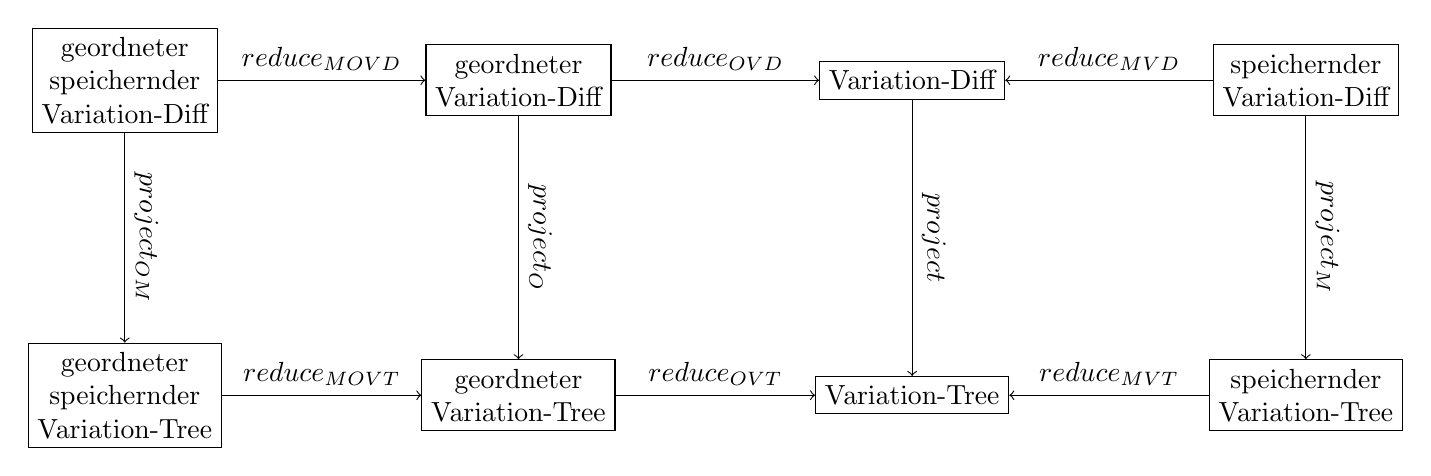
\begin{tikzpicture}
		\node[draw,align=center] (E) at (0,0) {geordneter\\speichernder\\
			Variation-Diff};
		\node[draw,align=center] (F) at (0,-4) {geordneter\\speichernder\\
			Variation-Tree};
		\node[draw,align=center] (A) at (5,0) {geordneter\\
			Variation-Diff};
		\node[draw,align=center] (B) at (5,-4) {geordneter\\
			Variation-Tree};
		\node[draw,align=center] (C) at (10,0) {Variation-Diff};
		\node[draw,align=center] (D) at (10,-4) {Variation-Tree};
		\node[draw,align=center] (G) at (15,0) {speichernder\\
			Variation-Diff};
		\node[draw,align=center] (H) at (15,-4) {speichernder\\
			Variation-Tree};
		\draw[->] (A) -- (B)  node[midway,sloped,above] {$project_O$} ;
		\draw[->] (C) -- (D)  node[midway,sloped,above] {$project$} ;
		\draw[->] (A) -- (C)  node[midway,sloped,above] {$reduce_{OVD}$} ;
		\draw[->] (B) -- (D)  node[midway,sloped,above] {$reduce_{OVT}$} ;
		\draw[->] (E) -- (F)  node[midway,sloped,above] {$project_{OM}$} ;
		\draw[->] (E) -- (A)  node[midway,sloped,above] {$reduce_{MOVD}$} ;
		\draw[->] (F) -- (B)  node[midway,sloped,above] {$reduce_{MOVT}$} ;
		\draw[->] (G) -- (H)  node[midway,sloped,above] {$project_{M}$} ;
		\draw[->] (G) -- (C)  node[midway,sloped,above] {$reduce_{MVD}$} ;
		\draw[->] (H) -- (D)  node[midway,sloped,above] {$reduce_{MVT}$} ;
	\end{tikzpicture}
	}
	\caption{Transformationen von verschiedenen Variation-Trees und Variation-Diffs}
\end{figure}
Mit der Erweiterung der Definitionen oder den Heuristiken können wir den Inhalt der Zeile mit \#endif bekommen und damit ist dieser Informationsverlust auch beseitigt.\\

Als Letztes müssen wir uns damit befassen, wie wir den Inhalt der Zeilen bekommen. Der Definition von Label nach werden dort entweder ein Implementierungsartefakt oder eine aussagenlogische Formel gespeichert. Ein Implementierungsartefakt kann dabei mehr als nur die Codezeile sein. Ein Implementierungsartefakt ist dabei  eine identifizierbare Einheit mit beliebiger Granularität innerhalb eines Softwareprojekts~\cite{BTS+:ESECFSE22}. Dazu sind Bedingungen in if-Anweisungen sind nicht immer als aussagenlogische Formeln gegeben und werden deshalb mithilfe von boolean abstraction in solche umgewandelt~\cite{BTS+:ESECFSE22}. Das kann z.B so aussehen: \#if A(x) > 3 ist gegeben und nach boolean abstraction sieht es dann so aus \#if A\_\_LB\_\_x\_\_RB\_\_GT\_\_3 . Dabei ist eine zurück Umwandlung nicht garantiert, da wir nicht sicher sein können das z.B  A\_\_LB\_\_x\_\_RB\_\_GT\_\_3 nicht als ein Variablenname gewählt wurde und damit keine Umwandlung benötigt. Unsere Arbeit ist darauf ausgelegt, dass wir einen Unparser bereitstellen, welcher aus Variation-Trees bzw. Variation-Diffs mit C-Präprozessor-Annotierten Code bzw. textbasiertes Diff erstellt. Aus diesem Grund, das wie so spezialisiert sind, fordern wir das Label als Implementierungsartefakt die Codezeile abspeichert und die aussagenlogischen Formeln trotzt dem boolean abstraction sich zu if-Bedingungen invertieren lassen. Mit diesen Forderungen beseitigen wir auch den letzten Informationsverlust.\\

Nachdem wir herausgefunden haben, welche für das Unparsen relevante Information verloren geht und wie man diese Information Zurück bekommen kann, sind wir in der Lage das alles zu nutzen, um einen Algorithmus zum Unparsen zu entwickeln.


\section{Unparsing}

%Im Baum stellen Knoten Blöcke dar, Tiefensuche geht alle blöcke eiser zweigt zuerst durch dann zum nächsten so entsteht wieder der Text


Nachdem wir festgestellt haben welche Informationen während des Parsens verlorengehen, müssen wir einen weg finden diese Informationen zurück zu bekommen und das Unparsen zu bewerkstelligen. Darüber geht es in dem folgenden Unterkapitel. Wir stellen unseren Algorithmus für das Unparsen von Variation-Trees und ein Vorgehen zum Unparsen von Variation-Diffs.\\

Damit unser Algorithmus korrekt funktioniert müssen paar Sachen beachtet werden. Als erstes gehen wir davon aus das die Reihenfolge der Knoten auch die Reihenfolge der Zeilen in dem Ergebnis des Unparsers widerspiegelt. Wenn ein Kindknoten A vor dem Kindknoten B aufgelistet wird bedeutet, dass das der Inhalt alle Knoten die einen Teilbaum mit Kindknoten A als Wurzel bilden vor dem Inhalt des Kindknoten B kommt. Als zweites muss man beachtet das Variation-Trees und Variation-Diffs keine Speicherung der Information über \#endif vorsehen. Unser Algorithmus kann zwar bestimmen an welchen Stellen ein \#endif kommen soll, aber er kann nicht die genauere Entfernung von Zeilenanfang wissen. Aus diesem Grund muss man hier entweder mit einer Heuristik arbeiten oder die Implementierung von Variation-Tree und Variation-Diff so modifizieren das diese Informationen gespeichert werden und wenn benötigt abgerufen.


\begin{algorithm}[H]
	\SetAlgoLined
	\DontPrintSemicolon
	\KwData{ein Vatiation-Tree}
	\KwResult{ein mit C-Präprozessor-Annotierten Code}
	initialisiere einen leeren Stack/Keller $stack$\;
	initialisiere einen String $ergebniss$
	$root$ $\leftarrow$ Variation-Tree gibt Wurzelknoten aus\;
	$kinder$ $\leftarrow$ $root$ gibt seine Kinderknoten aus\;
	\For{i = n $\to$ 1 }{
		lege den Knoten aus $kinder$[i] auf den Stack $stack$\;
	}
	\While{$stack$ nicht leer ist}{
		$knoten$ $\leftarrow$ nehme das oberste Element aus dem Stack $stack$\;
		\eIf{Knoten von Typ if oder elif}{
			modifiziere die gespeicherte Zeile aus $knoten$ so das in der Bedingung logische Zeichen durch äquivalente aus der Programmiersprache ersetzt werden und füge die den $ergebniss$ hinzu\;
		}{
			füge die gespeicherte Zeile aus $knoten$ den $ergebniss$ hinzu\;
		}
		
		\If{wenn knoten nicht von Typ Artefact ist und sein letztes Kindknoten nicht von Typ else oder elif ist}{
			erstelle einen Dummyknoten welcher die endif-Anweisung beinhaltet\;
			füge diesen Knoten den Stack hinzu\;
		}
		$kinder$ $\leftarrow$ $knoten$ gibt seine Kinderknoten aus\;
		\For{i = n $\to$ 1 }{
			lege den Knoten aus $kinder$[i] auf den Stack $stack$\;
		}
	}
	\caption{Ein Variation-Tree zum mit C-Präprozessor-Annotierten Code unparsen}
\end{algorithm}

\resizebox{0.95\textwidth}{0.7\textheight}{
\begin{tikzpicture}
	\node[draw,rectangle split,rectangle split parts=2,align=left] (A) at (0,0) {
			\begin{tikzpicture}
				\node[draw,diamond,fill=lightgray,thick] {root}
				child {node[draw,circle,thick] {a1}}
				child {node[draw,rectangle,thick] {\textbf{if} b1}
					child {node[draw,rectangle,thick] {\textbf{if} b2}
						child { node[draw,circle,thick] {a2}}
						child { node[draw,rectangle,thick] {\textbf{else}}
							child { node[draw,circle,thick] {a3}}
						}
					}
					child { node[draw,circle,thick] {a4}}
				};
				\draw [>=stealth,red,<-,line width=1mm] (0.9,-0.2) -- (1.5,-0.5);
				\node[rectangle split, rectangle split parts=3,draw, anchor=center] at (2.5,0) {\nodepart{two} a1 \nodepart{three} \textbf{if} b1};
			\end{tikzpicture}
	\nodepart{two} {\textbf{Ausgabe :}}};
	
	\node[draw,rectangle split,rectangle split parts=2,align=left] (B) at (5.5,0) {
		\begin{tikzpicture}
			\node[draw,diamond,fill=lightgray,thick] {root}
			child {node[draw,circle,thick] {a1}}
			child {node[draw,rectangle,thick] {\textbf{if} b1}
				child {node[draw,rectangle,thick] {\textbf{if} b2}
					child { node[draw,circle,thick] {a2}}
					child { node[draw,rectangle,thick] {\textbf{else}}
						child { node[draw,circle,thick] {a3}}
					}
				}
				child { node[draw,circle,thick] {a4}}
			};
			\draw [>=stealth,red,<-,line width=1mm] (-0.9,-0.9) -- (-1,-0.3);
			\node[rectangle split, rectangle split parts=2,draw, anchor=center] at (2.5,0) {\nodepart{two}\textbf{if} b1};
		\end{tikzpicture}
		\nodepart{two} \textbf{Ausgabe :}\\ Anweisung1 (a1)};

	\node[draw,rectangle split,rectangle split parts=2,align=left] (C) at (11,0) {
		\begin{tikzpicture}
			\node[draw,diamond,fill=lightgray,thick] {root}
			child {node[draw,circle,thick] {a1}}
			child {node[draw,rectangle,thick] {\textbf{if} b1}
				child {node[draw,rectangle,thick] {\textbf{if} b2}
					child { node[draw,circle,thick] {a2}}
					child { node[draw,rectangle,thick] {\textbf{else}}
						child { node[draw,circle,thick] {a3}}
					}
				}
				child { node[draw,circle,thick] {a4}}
			};
			\draw [>=stealth,red,<-,line width=1mm] (1,-0.9) -- (1.5,0);
			\node[rectangle split, rectangle split parts=4,draw, anchor=center] at (2.5,0) {\nodepart{two}\textbf{if} b2 \nodepart{three} a4 \nodepart{four}\textbf{endif}};
		\end{tikzpicture}
		\nodepart{two} \textbf{Ausgabe :}\\ Anweisung1 (a1) \\ \textbf{\#if} Bedingung1 (b1)};


	\node[draw,rectangle split,rectangle split parts=2,align=left] (D) at (17,0) {
		\begin{tikzpicture}
			\node[draw,diamond,fill=lightgray,thick] {root}
			child {node[draw,circle,thick] {a1}}
			child {node[draw,rectangle,thick] {\textbf{if} b1}
				child {node[draw,rectangle,thick] {\textbf{if} b2}
					child { node[draw,circle,thick] {a2}}
					child { node[draw,rectangle,thick] {\textbf{else}}
						child { node[draw,circle,thick] {a3}}
					}
				}
				child { node[draw,circle,thick] {a4}}
			};
			\draw [>=stealth,red,->,line width=1mm] (-0.5,-2) -- (-0.2,-2.7);
			\node[rectangle split, rectangle split parts=6,draw, anchor=center] at (2.5,-0.6) {\nodepart{two} a2 \nodepart{three} \textbf{else} \nodepart{four} \textbf{endif} \nodepart{five}a4 \nodepart{six} \textbf{endif}};
		\end{tikzpicture}
		\nodepart{two} \textbf{Ausgabe :}\\ Anweisung1 (a1) \\ \textbf{\#if} Bedingung1 (b1) \\ \hspace*{5mm}\textbf{\#if} Bedingung2 (b2)};
		
		
	\node[draw,rectangle split,rectangle split parts=2,align=left] (E) at (0,-11) {
		\begin{tikzpicture}
			\node[draw,diamond,fill=lightgray,thick] {root}
			child {node[draw,circle,thick] {a1}}
			child {node[draw,rectangle,thick] {\textbf{if} b1}
				child {node[draw,rectangle,thick] {\textbf{if} b2}
					child { node[draw,circle,thick] {a2}}
					child { node[draw,rectangle,thick] {\textbf{else}}
						child { node[draw,circle,thick] {a3}}
					}
				}
				child { node[draw,circle,thick] {a4}}
			};
			\draw [>=stealth,red,->,line width=1mm] (-0.9,-3.4) -- (-0.8,-4);
			\node[rectangle split, rectangle split parts=5,draw, anchor=center] at (2.5,-0.6) {\nodepart{two}\textbf{else} \nodepart{three} \textbf{endif} \nodepart{four} a4 \nodepart{five}\textbf{endif}};
		\end{tikzpicture}
		\nodepart{two} \textbf{Ausgabe :}\\ Anweisung1 (a1) \\ \textbf{\#if} Bedingung1 (b1) \\ \hspace*{5mm}\textbf{\#if} Bedingung2 (b2) \\ \hspace*{5mm}Anweisung2 (a2)};	
			
			
	\node[draw,rectangle split,rectangle split parts=2,align=left] (F) at (5.5,-11) {
		\begin{tikzpicture}
			\node[draw,diamond,fill=lightgray,thick] {root}
			child {node[draw,circle,thick] {a1}}
			child {node[draw,rectangle,thick] {\textbf{if} b1}
				child {node[draw,rectangle,thick] {\textbf{if} b2}
					child { node[draw,circle,thick] {a2}}
					child { node[draw,rectangle,thick] {\textbf{else}}
						child { node[draw,circle,thick] {a3}}
					}
				}
				child { node[draw,circle,thick] {a4}}
			};
			\draw [>=stealth,red,->,line width=1mm] (0.8,-3.4) -- (0.8,-4);
			\node[rectangle split, rectangle split parts=5,draw, anchor=center] at (2.5,-0.6) {\nodepart{two} a3 \nodepart{three} \textbf{endif} \nodepart{four} a4 \nodepart{five}\textbf{endif}};
		\end{tikzpicture}
		\nodepart{two} \textbf{Ausgabe :}\\ Anweisung1 (a1) \\ \textbf{\#if} Bedingung1 (b1) \\ \hspace*{5mm}\textbf{\#if} Bedingung2 (b2) \\ \hspace*{10mm}Anweisung2 (a2) \\ \hspace*{5mm}\textbf{\#else}};
		
	
	\node[draw,rectangle split,rectangle split parts=2,align=left] (G) at (11,-11) {
		\begin{tikzpicture}
			\node[draw,diamond,fill=lightgray,thick] {root}
			child {node[draw,circle,thick] {a1}}
			child {node[draw,rectangle,thick] {\textbf{if} b1}
				child {node[draw,rectangle,thick] {\textbf{if} b2}
					child { node[draw,circle,thick] {a2}}
					child { node[draw,rectangle,thick] {\textbf{else}}
						child { node[draw,circle,thick] {a3}}
					}
				}
				child { node[draw,circle,thick] {a4}}
			};
			\draw [>=stealth,red,->,line width=1mm] (1,-5) -- (0.9,-5.5);
			\node[rectangle split, rectangle split parts=4,draw, anchor=center] at (2.5,-0.6) {\nodepart{two} \textbf{endif} \nodepart{three} a4 \nodepart{four} \textbf{endif}};
		\end{tikzpicture}
		\nodepart{two} \textbf{Ausgabe :}\\ Anweisung1 (a1) \\ \textbf{\#if} Bedingung1 (b1) \\ \hspace*{5mm}\textbf{\#if} Bedingung2 (b2) \\ \hspace*{10mm}Anweisung2 (a2) \\ \hspace*{5mm}\textbf{\#else} \\
		\hspace*{10mm}Anweisung3 (a3)};
		
	
	\node[draw,rectangle split,rectangle split parts=2,align=left] (H) at (17,-11) {
		\begin{tikzpicture}
			\node[draw,diamond,fill=lightgray,thick] {root}
			child {node[draw,circle,thick] {a1}}
			child {node[draw,rectangle,thick] {\textbf{if} b1}
				child {node[draw,rectangle,thick] {\textbf{if} b2}
					child { node[draw,circle,thick] {a2}}
					child { node[draw,rectangle,thick] {\textbf{else}}
						child { node[draw,circle,thick] {a3}}
					}
				}
				child { node[draw,circle,thick] {a4}}
			};
			\node[rectangle split, rectangle split parts=3,draw, anchor=center] at (2.5,-0.6) {\nodepart{two} a4 \nodepart{three} \textbf{endif} };
		\end{tikzpicture}
		\nodepart{two} \textbf{Ausgabe :}\\ Anweisung1 (a1) \\ \textbf{\#if} Bedingung1 (b1) \\ \hspace*{5mm}\textbf{\#if} Bedingung2 (b2) \\ \hspace*{10mm}Anweisung2 (a2) \\ \hspace*{5mm}\textbf{\#else} \\
		\hspace*{10mm}Anweisung3 (a3) \\ \hspace*{5mm}\textbf{\#endif}};
		
		
		
	\node[draw,rectangle split,rectangle split parts=2,align=left,rectangle split horizontal] (I) at (2.5,-22) {
		\begin{tikzpicture}
			\node[draw,diamond,fill=lightgray,thick] {root}
			child {node[draw,circle,thick] {a1}}
			child {node[draw,rectangle,thick] {\textbf{if} b1}
				child {node[draw,rectangle,thick] {\textbf{if} b2}
					child { node[draw,circle,thick] {a2}}
					child { node[draw,rectangle,thick] {\textbf{else}}
						child { node[draw,circle,thick] {a3}}
					}
				}
				child { node[draw,circle,thick] {a4}}
			};
			\draw [>=stealth,red,->,line width=1mm] (2,-1.5) -- (1.7,-2.5);
			\node[rectangle split horizontal=false, rectangle split parts=2,draw] at (2.5,-0.6) {\nodepart{two}  \textbf{endif} };
		\end{tikzpicture}
		\nodepart{two} \textbf{Ausgabe :}\\ Anweisung1 (a1) \\ \textbf{\#if} Bedingung1 (b1) \\ \hspace*{5mm}\textbf{\#if} Bedingung2 (b2) \\ \hspace*{10mm}Anweisung2 (a2) \\ \hspace*{5mm}\textbf{\#else} \\
		\hspace*{10mm}Anweisung3 (a3) \\ \hspace*{5mm}\textbf{\#endif} \\ \hspace*{5mm} Anweisung4 (a4) };
		
		
	\node[draw,rectangle split,rectangle split parts=2,align=left,rectangle split horizontal] (J) at (13,-22) {
		\begin{tikzpicture}
			\node[draw,diamond,fill=lightgray,thick] {root}
			child {node[draw,circle,thick] {a1}}
			child {node[draw,rectangle,thick] {\textbf{if} b1}
				child {node[draw,rectangle,thick] {\textbf{if} b2}
					child { node[draw,circle,thick] {a2}}
					child { node[draw,rectangle,thick] {\textbf{else}}
						child { node[draw,circle,thick] {a3}}
					}
				}
				child { node[draw,circle,thick] {a4}}
			};
			\node[rectangle split, rectangle split parts=1,draw] at (2.5,-0.6) {    };
		\end{tikzpicture}
		\nodepart{two} \textbf{Ausgabe :}\\ Anweisung1 (a1) \\ \textbf{\#if} Bedingung1 (b1) \\ \hspace*{5mm}\textbf{\#if} Bedingung2 (b2) \\ \hspace*{10mm}Anweisung2 (a2) \\ \hspace*{5mm}\textbf{\#else} \\
		\hspace*{10mm}Anweisung3 (a3) \\ \hspace*{5mm}\textbf{\#endif} \\ \hspace*{5mm} Anweisung4 (a4) \\ \textbf{\#endif}};
\end{tikzpicture}
}

\section{Laufzeitanalyse}
\subsection{Laufzeitanalyse für Unparsen von Variation-Trees}

\subsection{Laufzeitanalyse für Unparsen von Variation-Diffs}








